\subsection{CMA micro-benchmark on Broadwell and TX2}
\label{sec:pa-microbenchmark}
In this subsection we will introduce the CMA\_appinv micro-benchmark and present performance results from tests on the Intel Broadwell and Cavium ARM-based ThunderX2 architectures.
In addition we compare performance of the micro-benchmark when built with different compilers and runtime libraries.

%Isambard is a XC50 system hosted by the Met Office and funded by the GW4 alliance and EPSRC.
%The heterogeneous system contains chips of various architectures including 164 Cavium ThunderX2 nodes.

\subsubsection{CMA micro-benchmark}

The GungHo dynamical model performs operations to solve
\begin{equation} \label{eq:matvec}
A \cdot \mathbf{x} = \mathbf{b}
\end{equation}
in various guises and contexts where $A$ is a matrix representing a partial differential equation, $\mathbf{b}$ is a vector containing information describing boundary conditions and $\mathbf{x}$ is a state vector.
The finite element methods that the GungHo application uses are written to perform operations on a cell-by-cell basis in what is termed Local Matrix Assembly (LMA).
The LMA micro-benchmark discussed in Section \ref{sec:pa} is a characteristic example of such methods.
The LFRic infrastructure also contains methods for solving equation \ref{eq:matvec} on a column-by-column basis.
Although these Column Matrix Assembly (CMA) methods have yet to be utilised by the full GungHo application they are deployed in the gravity\_wave mini-app.

For this report we generated a new CMA micro-benchmark using LFRic revision 15378 focused on the columnwise\_op\_appinv\_kernel\_code() routine in the gravity\_wave mini-app.
This kernel is used in the pre-conditioner for the Helmholtz solver to solve the tridiagonal case of equation \ref{eq:matvec} using the Thomas Algorithm.
As per the LMA micro-benchmark, the driver code was extracted from the Psyclone-generated Psy-layer and the kernel was taken directly from the LFRic source code.
By design, the driver routine contains the so called global optimisations, namely OpenMP worksharing and colouring (to prevent data race conditions) over columns on the sphere.

The dinodump capability from PYSKE was used to generate Known Good Output (KGO) which we use to verify the micro-benchmark behaved as expected in later tests.
This involved adding additional PSYKE subroutine calls to the Psy-layer code in the gravity\_wave mini-app in order to capture the input scalars and arrays for the kernel.
The micro-benchmark driver code was also trivially modified to read in the produced dinodump before calling the kernel and compare the result of the kernel against the KGO.
Before running the mini-app to generate the dinodumo the number of vertical layers in the configuration was modified from the default (10) to 256.
While current NWP and climate GA and RA production configurations use between 70 and 90 vertical (UM) levels we took 256 layers in order to increase the throughput of the benchmark and also in expectation that future configurations will run with increased vertical resolution.


While generating the new micro-benchmark a minor bug in kernel was discovered.
Specifically, the manner in which the kernel is called in gravity\_wave mini-app (and the supporting code comments) indicate that the kernel is called to update the target array but instead the kernel actually populates the array while overriding the initial contents.
It was confirmed by the original author of the code that the functionality of the kernel was correct and the comments are in error.
The bug has minimal performance impact on CPU architectures- an intent(inout) array should be intent(out)- but may have a larger impact on GPU architectures where the array would be being offloaded unnecessarily. 

The resultant micro-benchmark can be found in the micro-benchmark ~\cite{lfric-microbenchmarks} suite on github.
We note that the LMA and CMA\_appinv micro-benchmarks serve different purposes in the solver code and as such direct comparisons are not appropriate.

\subsubsection{CMA\_appinv performance}

We present timings for the kernel on Intel Broadwell and Cavium ThunderX2 as measured using omp\_get\_wtime().
In each case the kernel was run for 1000 iterations in order to obtain a smooth out runtime variability.
We use the latest stable version of each compiler available on the two platforms at the time of writing.
Each executable was built with the -O3 optimisation flag.

\begin{figure}
\centering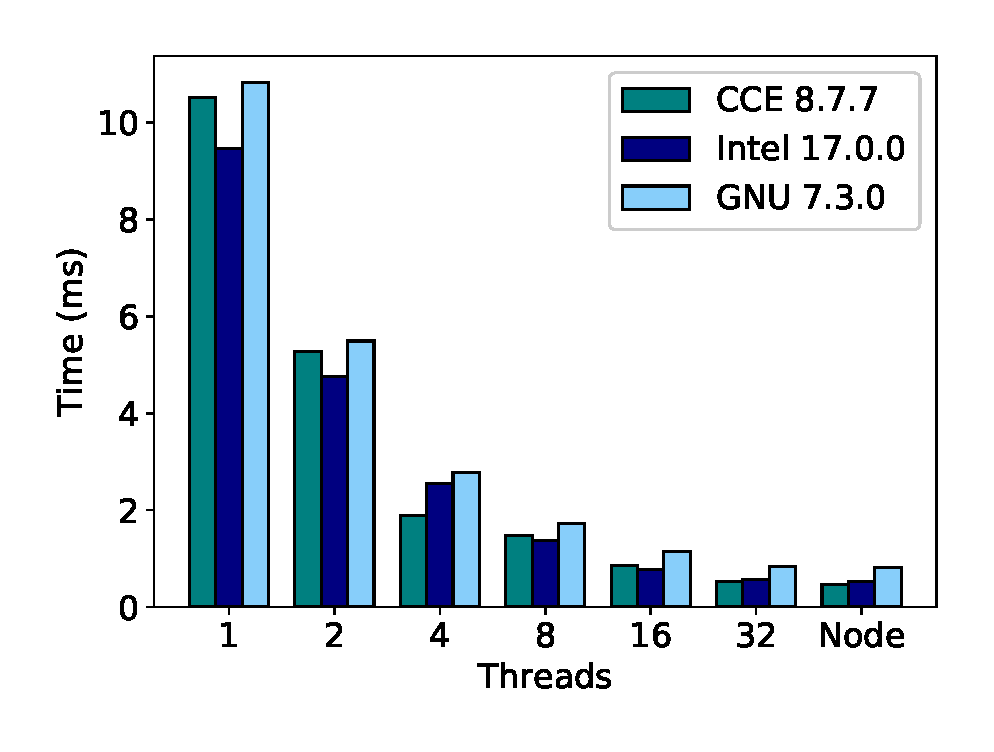
\includegraphics[scale=0.5]{figs/Broadwell_microbenchmark_vanilla.eps}
\caption{Thread-scaling of runtime on a Broadwell node. A lower time is better.}
\end{figure}

\begin{figure}
\centering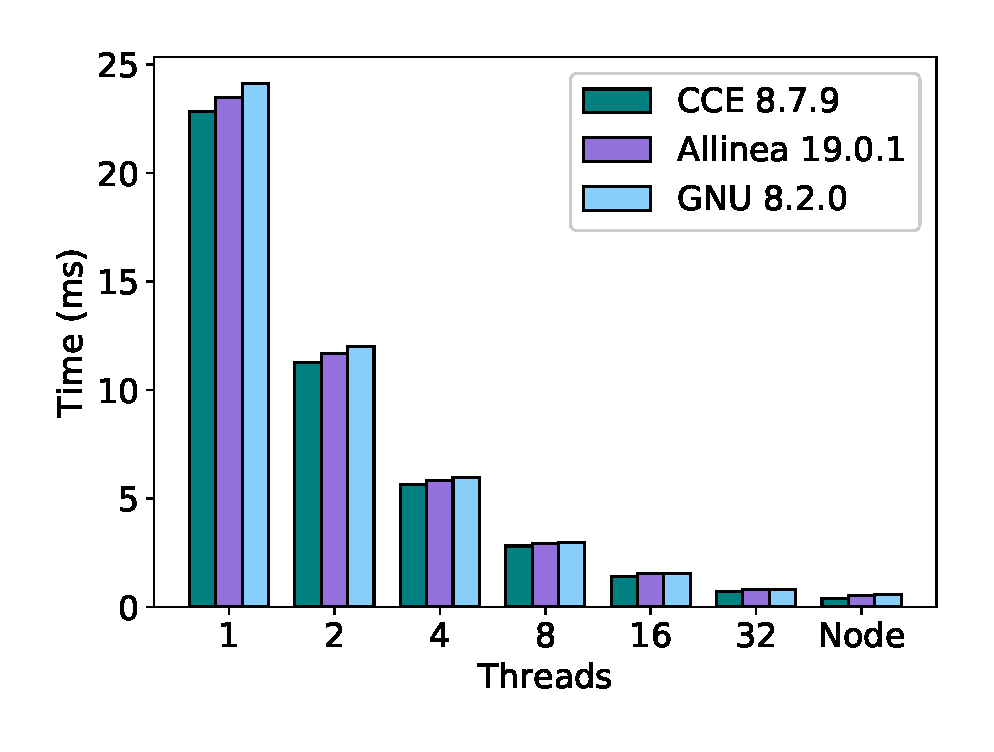
\includegraphics[scale=0.5]{figs/ThunderX2_microbenchmark_vanilla.eps}
\caption{Thread-scaling of runtime on a ThunderX2 node. A lower time is better.}
\end{figure}

\paragraph{Intel Broadwell} is the architecture in use for production NWP systems on the Met Office XC40 system.
Each node includes two 18-core 2.1 GHz processors.
On the XCS platform the compilers used were
\begin{itemize}
\item CCE 8.7.7
\item Intel 17.0.0.098
\item GNU 7.3.0
\end{itemize}

During the development of this work we encountered notable differences in performance between compiler versions.
For example, a measurable performance degradation between cce 8.6.0 and the cce 8.7.x series.
The single threaded (OMP\_NUM\_THREADS=1) runtime increased from 7.4s to 10.5s when changing between the two versions.
In other words cce 8.6.0 produces a faster single-threaded executable than the Intel compiler but the 8.7.7 executable is slower than the Intel generated version.
This discrepancy is outwith the observed run-to-run variability on the system and is unexplained at present.
We use the more recent (but slightly less performant) cce 8.7.7.

\paragraph{Cavium ThunderX2} processors, unlike some other ARM-based architectures, are targeted at the HPC market.
Each Isambard node includes two 32-core 2.1GHz processors: i.e. 64 cores per node vs the 36 cores of the Intel Broadwell nodes on XCS.
At the time of writing (after the March 2019 upgrade to CLE7.0) the supported compilers on the ARM-based nodes are
\begin{itemize}
\item CCE 8.7.9
\item Allinea 19.0.1
\item GNU 8.2.0
\end{itemize}
where the Allinea compiler is built on top of LLVM and Flang.

% single threaded performance on TX2 is notably lower.
% thread scaling wins out for TX2. There are enough columns of cells to keep all the threads busy.


\subsubsection{CMA\_appinv performance using drop-in library call}
Next we investigate whether the implementation of the Thomas algorithm as written in the kernel can be replaced with a call to a standard library- in this case LAPACK.
The potential benefits of this include a potential improvement to runtimes of current architectures.
But, more importantly calling a standard API allows us to tap into routines that have been optimised specifically for the architecture being used.
This could provide performance portability while reducing porting and maintenance costs when moving between future compute platforms.
A potential problem with this plan is that the memory layout used in the columnwise operator type objects differs from that expected by the LAPACK API.

The version of the micro-benchmark used can be found in a branch of the github repo.

Thread scaling
Thread-scales OK but runtime is poor.
Is it memory copies? No, we tried taking these out but couldn't match ``vanilla'' performance.

\subsubsection{Discussion}

It is worth noting that there are few opportunities for vectorisation in the current implementation.

In avoiding building the LFRic infrastructure we also avoid compiler support problems.
TX2 vs Broadwell
Single thread performance on Broadwell is comfortably better than TX2. However, when multithreading is considered then the machines are node-for-node comparable.
Use of drop-in lib
Use of LAPACK as a drop-in replacement for kernel. Not optimal at present- LAPACK is optimised for larger problems.

Worth investigating vectorised versions of the algorithm, especially in the context of GPUs.
